\documentclass[]{article}
\usepackage[T1]{fontenc}
\usepackage[utf8]{inputenc}
\usepackage[swedish]{babel}
\usepackage[margin=1.7in]{geometry}
\usepackage{mathtools}
\usepackage{graphicx}
\usepackage{listings}



%opening
\title{DD1350 Logik för dataloger \\ Laboration 2}
\author{Erik Ringdahl, erikrin@kth.se \\ Joel Tjärnstig, joelt@kth.se}

\begin{document}

\setlength\parindent{0pt}
\maketitle

\section{Verktygsutveckling}
Programmet börjar med att läsa in modellen, sanningstilldelningslistan, starttillståndet samt formeln. Dessa värden skickas sedan in i ett predikat \texttt{check} tillsammans med en tom lista som håller reda på vilka tillstånd vi har besökt. check verifierar varje delformel rekursivt och börjar innerst. För att göra detta använder check sig av två hjälppredikat, \texttt{check\_all} som rekursivt kollar A-formler, samt \texttt{check\_exist} som rekursivt kollar E-formler.

\clearpage
\section{Modellering}
Vi valde att modellera en förenklad uttagsautomat. En användare möts först av en välkomstskärm. Användaren verifieras genom att ange sin pinkod. Om pinkoden är fel, bes användaren ange den igen. Om användaren anger rätt pinkod får ett belopp anges. Om beloppet inte kan tas ut får användaren skriva ett nytt belopp. Om beloppet finns tillgängligt tas pengarna ut och uttagsautomaten återgår till välkomstskärmen. Användaren kan även närsomhelst avbryta uttaget och återgå till välkomstskärmen.

\subsection{Tillståndsgraf}
Vi har 5 olika tillstånd (\textbf{Welcome Screen, Verify, Retry, Select Amount, Withdraw Money}) och 4 atomer (\texttt{Pin Entered, Failed, Verified, Valid Amount}).

\begin{figure}[h]
\centering
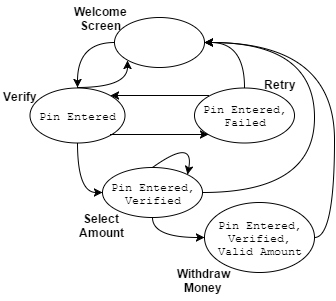
\includegraphics[width=0.75\linewidth]{modell}
\caption{Tillståndsgraf för uttagsautomat}
\label{fig:modell}
\end{figure}

\clearpage
\subsection{Prolog-kompatibel representation}
\begin{verbatim}
% States are ws(welcome screen), ve(verify), re(retry), 
% sa(select amount) and wm(withdraw money).
[
 [ws, [ve]],
 [ve, [ws, ve, re, sa]],
 [re, [ws, ve]],
 [sa, [ws, sa, wm]],
 [wm, [ws]]
].

% Labeling
[
 [ws, []],
 [ve, [pe]],
 [re, [pe, f]],
 [sa, [pe, v]],
 [wm, [pe, v, va]]
].
\end{verbatim}

\clearpage
\section{Specifiering}

\subsection{Hållbar systemegenskap}
Det finns en stig där så småningom det går att ta ut pengar.\\
\texttt{ef(and(and(pe,v),va))}

\subsection{Ohållbar systemegenskap}
Det finns en stig där något av nästa steg inte är välkomstskärmen.\\
\texttt{ef(not(ex(not(pe))))}

\section{Predikat}
\begin{description}
	\item[\texttt{verify -}] sant när bevisfilen kan läsas på ett korrekt sätt samt när formeln är sann.
	
	\item[\texttt{check -}] sant när formeln samt alla underliggande rekursiva anrop är sanna.
	
	\item[\texttt{check\_all -}] sant då basfallet gäller, dvs när grannlistan är tom. Eller när formeln gäller för alla grannar i listan.
	
	\item[\texttt{check\_exist -}] sant då basfallet inte gäller, dvs när grannlistan inte är tom. Eller när formeln gäller för någon granne i listan.
	
	\end{description}

\section{Verifiering}
\subsection{Systemegenskaper}
\begin{description}
	\item[Hållbar] Eftersom det finns en stig där \texttt{pe,v,a} kommer att vara sanna, nämligen i \texttt{ws} ska egenskapen returnera sant, vilket den gjorde.
	
	\item[Ohållbar] Eftersom alla tillstånd kan gå över till \texttt{ws} alltså då \texttt{pe} inte är sann ska egenskapen returnerna falskt, vilket den gjorde.
\end{description}

\subsection{Givna Testfall}
Modellproveraren klarade samtliga 732 givna testfall.

\clearpage
\section*{Appendix}
\appendix

\section{Källkod}

%\lstinputlisting[language=Prolog]{../modelcheck.pl}



\end{document}